\chapter{Implementation et Configuration}

\section{Deploiement de l'Infrastructure}

\subsection{Environnement de Laboratoire}

\subsubsection{Architecture de Test}

L'environnement de laboratoire a ete concu pour reproduire fidelement l'ecosysteme hospitalier tout en permettant des tests d'intrusion controles.

\begin{table}[H]
    \centering
    \caption{Mapping de l'environnement de laboratoire}
    \begin{tabular}{|l|l|c|l|}
        \hline
        \textbf{Segment} & \textbf{Reseau}  & \textbf{Role}             & \textbf{Composants}     \\
        \hline
        Production       & 192.168.15.0/24  & Environnement hospitalier & SIH, PACS, Workstations \\
        \hline
        Attaquant        & 192.168.183.0/24 & Red Team                  & Kali Linux, Metasploit  \\
        \hline
        SIEM/SOAR        & 192.168.3.0/24   & Blue Team                 & Wazuh, TheHive, Cortex  \\
        \hline
        Internet         & 192.168.3.0/24   & Simulation WAN            & Malicious websites      \\
        \hline
        Defense          & 192.168.181.0/24 & Firewall                  & pfSense , modsecurity   \\
        \hline
    \end{tabular}
\end{table}

\subsubsection{Scenarios de Simulation}

\paragraph{Environnement Hospitalier Simule}
\begin{enumerate}
    \item \textbf{Serveur SIH} (192.168.15.10)
          \begin{itemize}
              \item Windows Server 2019 avec IIS
              \item Application web de gestion patient
              \item Base de donnees SQL Server
              \item Partages SMB pour documents medicaux
          \end{itemize}

    \item \textbf{Serveur PACS} (192.168.15.20)
          \begin{itemize}
              \item Windows Server 2016 vulnerable (MS17-010)
              \item Service DICOM pour imagerie medicale
              \item Stockage d'images radiologiques
              \item Protocoles non chiffres (test)
          \end{itemize}

    \item \textbf{Postes Utilisateurs} (192.168.15.30-50)
          \begin{itemize}
              \item Windows 10 avec agents Wazuh
              \item Applications medicales courantes
              \item Navigateurs web (tests XSS)
              \item Acces reseau standard
          \end{itemize}
\end{enumerate}

\paragraph{Infrastructure d'Attaque}
\begin{enumerate}
    \item \textbf{Kali Linux Attacker} (192.168.183.2)
          \begin{itemize}
              \item Framework Metasploit pour EternalBlue
              \item Outils de scan reseau (Nmap, Masscan)
              \item Payloads personnalises
              \item Scripts d'automatisation d'attaque
          \end{itemize}

\end{enumerate}

\subsection{Configuration Wazuh SIEM}

\subsubsection{Deploiement Architecture Distribuee}


\begin{lstlisting}[style=xmlstyle,caption=Configuration Wazuh Manager principal]
<!-- /var/ossec/etc/ossec.conf -->
<ossec_config>
  <global>
    <jsonout_output>yes</jsonout_output>
    <alerts_log>yes</alerts_log>
    <logall>no</logall>
    <logall_json>no</logall_json>
    <email_notification>yes</email_notification>
    <smtp_server>smtp.hospital.local</smtp_server>
    <email_from>soc@hospital.local</email_from>
    <email_to>admin@hospital.local</email_to>
    <hostname>wazuh-manager</hostname>
    <email_maxperhour>100</email_maxperhour>
  </global>
<!-- other config  -->
  <command>
    <name>disable-network</name>
    <executable>disable-network.cmd</executable> 
    <timeout_allowed>yes</timeout_allowed>
  </command>

  <integration>
    <name>custom-dns-integration</name>
    <hook_url>http://sbihi.soar.ma:5678/webhook/wazuh-sysmon</hook_url>
    <level>3</level>
    <group>sysmon_event_22</group>
    <alert_format>json</alert_format>
  </integration>
<!-- other config  -->

</ossec_config>
\end{lstlisting}

\subsection{Regles de Detection Personnalisees}

\begin{lstlisting}[style=xmlstyle,caption=Regles EternalBlue specialisees pour environnement hospitalier]
<!-- /var/ossec/etc/rules/100_hospital_eternalblue.xml -->
<group name="eternalblue,hospital,critical">
  
  <!-- Phase 1: SMB Port Scanning -->
  <rule id="100010" level="5">
    <decoded_as>windows-eventlog</decoded_as>
    <field name="win.system.eventID">^5156$</field>
    <field name="win.eventdata.destinationPort">^445$</field>
    <regex>192\.168\.183\.</regex>
    <description>EternalBlue: SMB port scan from external network to hospital systems</description>
    <group>attack.discovery,attack.t1046</group>
    <options>no_full_log</options>
  </rule>
  <!-- Phase 2: SMBv1 Negotiate Attempt -->
  <rule id="100011" level="8">
    <if_sid>100010</if_sid>
    <same_source_ip />
    <description>EternalBlue: SMBv1 negotiate attempt after port scan</description>
    <group>attack.initial_access,attack.t1190</group>
  </rule>
  <!-- Phase 3: Exploit Buffer Overflow -->
  <rule id="100012" level="12">
    <if_matched_sid>100011</if_matched_sid>
    <same_source_ip />
    <regex>STATUS_BUFFER_OVERFLOW|STATUS_ACCESS_VIOLATION</regex>
    <description>EternalBlue: Buffer overflow exploitation detected - CRITICAL HOSPITAL ALERT</description>
    <group>attack.execution,attack.t1055</group>
  </rule>
  <!-- Phase 4: Payload Execution -->
  <rule id="100013" level="13">
    <if_matched_sid>100012</if_matched_sid>
    <same_source_ip />
    <field name="win.system.eventID">^1$</field>
    <regex>cmd\.exe|powershell\.exe|rundll32\.exe</regex>
    <description>EternalBlue: Malicious payload execution</description>
    <group>attack.execution,attack.persistence</group>
  </rule>
</group>
\end{lstlisting}


\subsection{Configuration ModSecurity WAF}

\subsubsection{Protection Applicative Web}

\paragraph{Configuration de Base}

\begin{lstlisting}[caption=Configuration ModSecurity pour applications medicales]
# /etc/modsecurity/hospital_medical_apps.conf

# Detection d'anomalies pour applications medicales
SecRule REQUEST_URI "@detectSQLi" \
    "id:1001,phase:2,block,\
     msg:'SQL Injection Attack in Medical Application',\
     logdata:'Matched Data: %{MATCHED_VAR} found in %{MATCHED_VAR_NAME}',\
     tag:'application-multi',tag:'medical-app',tag:'attack-sqli',\
     severity:'CRITICAL'"

# Protection XSS specialisee pour formulaires patient
SecRule ARGS "@detectXSS" \
    "id:1002,phase:2,block,\
     msg:'XSS Attack in Patient Data Form',\
     logdata:'Matched Data: %{MATCHED_VAR} found in %{MATCHED_VAR_NAME}',\
     tag:'application-multi',tag:'patient-data',tag:'attack-xss',\
     severity:'HIGH'"

# Limitation de debit pour prevenir DoS sur systemes critiques
SecRule IP:REQUEST_COUNT "@gt 50" \
    "id:1005,phase:1,deny,status:429,\
     msg:'Rate limiting: too many requests from single IP',\
     tag:'dos-protection',tag:'hospital-systems',\
     severity:'MEDIUM'"

\end{lstlisting}
\clearpage


\subsection{Configuration TheHive SOAR}

\subsubsection{Modele de Donnees Hospitalier}

\paragraph{Templates d'Incidents Medicaux}

\begin{lstlisting}[style=jsonstyle,caption=Template TheHive pour incident EternalBlue]
{
  'parameters': {
    'title': "EternalBlue Phase 1 - Initial Detection",
    'description': "**Initial EternalBlue exploitation attempt detected**\n\n**Attack Details:**\n- Source IP: {{ $json.body.source_ip }}\n- Target IP: {{ $json.body.destination_ip }}\n- Phase: {{ $json.body.attack_analysis.phase }}\n- Attack Status: {{ $json.body.attack_analysis.attack_status }}\n- Detection Time: {{ $json.body.processing_timestamp }}\n\n**Signature:** {{ $json.body.signature }}\n\n**Recommended Actions:**\n1. Monitor source IP for escalation\n2. Review target system logs\n3. Verify SMB service configurations\n4. Check for subsequent attack phases\n\n**Priority:** {{ $json.body.attack_analysis.priority_level }} - Enhanced monitoring required",
    'date': "={{ $json.body.timestamp }}",
    'tags': "=eternalblue,phase1,smb,exploitation-attempt",
    'type': "eternalblue",
    'source': "=suricata",
    'sourceRef': "={{ $json.body.timestamp }}",
    'additionalFields': {}
  },
}
\end{lstlisting}

\begin{itemize}
    \item \textbf{title} : Titre normalise de la phase d'attaque.
    \item \textbf{description} : Corps riche (Markdown) listant details techniques et actions recommandees.
    \item \textbf{date} : Horodatage source (timestamp de l'evenement original).
    \item \textbf{tags} : Mots cles facilitant la priorisation et la recherche (phase, protocole, type d'exploitation).
    \item \textbf{type} : Categorie fonctionnelle de l'incident (ici "eternalblue").
    \item \textbf{source} / \textbf{sourceRef} : Origine de l'alerte (moteur de detection) et identifiant de correlation.
    \item \textbf{additionalFields} : Conteneur extensible pour des meta‑donnees specifiques (initialement vide, peut recevoir criticite, SLA, proprietaire, etc.).
\end{itemize}

\paragraph{Workflows Automatises Specialises}

\paragraph{Workflow n8n pour reponse automatisee EternalBlue}

L'orchestration automatisee des reponses aux incidents EternalBlue est geree par un workflow n8n dedie, qui integre la detection Suricata avec la gestion d'incidents TheHive.


\textbf{Architecture du workflow :}
\begin{itemize}
    \item \textbf{Trigger} : Webhook HTTP POST depuis Suricata lors de detection EternalBlue
    \item \textbf{Creation de cas} : Generation automatique d'incident TheHive avec metadonnees hospitalieres
    \item \textbf{Reponse automatisee} : Actions de mitigation selon la criticite (isolation, blocage IP, notification medicale)
\end{itemize}

\textbf{Flux de traitement :}
\begin{enumerate}
    \item Reception de l'alerte Suricata via webhook
    \item Creation du cas TheHive avec observables
    \item Declenchement des actions de reponse appropriees
    \item Notification des equipes medicales
\end{enumerate}

\section{Integration des Composants}

\subsection{API Integration Layer}

\subsubsection{Integration Suricata-TheHive via Webhooks}

Pour la chaine EternalBlue, c'est \textbf{Suricata} qui assure la detection reseau (analyse SMB) et alimente l'automatisation. Deux scripts systeme orchestrent l'extraction PCAP, la correlation multi-phase et l'envoi d'alertes vers n8n / TheHive.

\paragraph{Scripts d'extraction et de correlation EternalBlue}
\begin{itemize}
    \item \texttt{Suricta/eternalblue\_soar\_unified.sh} : script unifie (v4.0) lisant \texttt{eve.json}, mappant les IDs de regles aux phases (PHASE\_1... PHASE\_3, CORRELATION\_*), dedoublonnant les sessions (suivi src/dst), analysant la progression, recherchant ou re-extrayant les PCAP (fenetre variable jusqu'a 60s), testant l'integrite (tcpdump), produisant une charge JSON enrichie (phase, statut, priorite) et envoyant un webhook HTTP vers n8n (variable \texttt{N8N\_WEBHOOK}).
    \item \texttt{Suricta/intelligent-extractor.service} : unit systemd demarrant le script apres \texttt{suricata.service}, assure redemarrage automatique et passe l'URL du webhook (Environment=). Garantit la resilience apres reboot.
\end{itemize}

\paragraph{Architecture d'integration}
\begin{itemize}
    \item \textbf{Suricata + Scripts} : Detection SMB + extraction / correlation + webhook JSON (EternalBlue).
    \item \textbf{Wazuh Webhooks} : Complement host / processus (autres familles d'incidents).
    \item \textbf{Workflows n8n} : Normalisation, enrichment (CTI, contexte asset) et routage.
    \item \textbf{API TheHive} : Creation de cas, ajout d'observables.
    \item \textbf{Cortex} : Analyse automatisee (hash, IP, URL) declenchee depuis TheHive.
\end{itemize}

\paragraph{Flux d'integration EternalBlue}
\begin{enumerate}
    \item Suricata genere une alerte (ID regle SMB) ecrite dans \texttt{eve.json}.
    \item \texttt{eternalblue\_soar\_unified.sh} corrige/associe la phase, met a jour la correlation, extrait ou re-utilise un PCAP.
    \item Le script envoie un webhook JSON vers n8n (phase, priorite, statut progression, chemin PCAP).
    \item n8n cree / met a jour un cas TheHive (template incident) et ajoute observables (IPs, signature SMB, hash PCAP si calcule).
    \item TheHive appelle Cortex pour enrichment (reputation IP, sandbox hash).
    \item n8n peut declencher un blocage (OPNsense alias) suivant la priorite.
\end{enumerate}

\paragraph{Configuration des endpoints}
\begin{itemize}
    \item \texttt{/webhook/eternalblue-alert} : Reception des webhooks Suricata (script extraction) vers n8n.
    \item \texttt{/webhook/xss}, : Flux Wazuh ou ModSecurity paralleles.
\end{itemize}

Cette approche combine detection reseau temps reel (Suricata) et logique SOAR (scripts + n8n + TheHive/Cortex) sans scripts Python lourds, tout en offrant une correlation multi-phase fiable et une reutilisation intelligente des PCAP pour minimiser la charge disque.

\subsubsection{Workflows n8n Specialises}

Le projet dispose de plusieurs workflows n8n pre-configures pour differents types d'incidents de securite :

\paragraph{Workflow XSS}
\texttt{ATTACK\_SCENARIOS/xss/n8n\_workflow.json}
\begin{itemize}
    \item Detection automatique des attaques XSS via ModSecurity
    \item Blocage automatique des IP malveillantes via OPNsense
    \item Integration avec l'API OPNsense pour mise a jour des alias de blocage
    \item Notification automatique des equipes de securite
\end{itemize}

\paragraph{Workflow Malicious Websites}
\texttt{ATTACK\_SCENARIOS/malicious\_websites/n8n\_workflow.json}
\begin{itemize}
    \item Surveillance des connexions vers des sites malveillants
    \item Correlation avec les bases de threat intelligence
    \item Actions de quarantaine pour les postes compromis
    \item Generation de rapports d'incident automatises
\end{itemize}

Ces workflows demontrent l'efficacite de l'approche SOAR pour l'automatisation des reponses aux incidents dans un environnement hospitalier, permettant une reaction rapide tout en respectant les contraintes operationnelles du secteur medical.

\section{Validation et Tests}

\subsection{Metriques de Performance}

Les tests de performance effectues sur l'infrastructure deployee montrent des resultats satisfaisants pour un environnement hospitalier :

\begin{table}[H]
    \centering
    \caption{Metriques de performance des composants SIEM/SOAR}
    \begin{tabular}{|l|c|c|c|}
        \hline
        \textbf{Composant} & \textbf{Latence moyenne} & \textbf{Debit} & \textbf{Disponibilite} \\
        \hline
        Wazuh Manager      & 50ms                     & 10k events/sec & 99.9\%                 \\
        \hline
        TheHive            & 200ms                    & 100 cases/min  & 99.8\%                 \\
        \hline
        Cortex Analyzers   & 2-30s                    & Variable       & 99.5\%                 \\
        \hline
        n8n Workflows      & 100ms                    & 500 req/min    & 99.9\%                 \\
        \hline
    \end{tabular}
\end{table}

\subsection{Scenarios de Test}

L'efficacite de la solution a ete validee a travers plusieurs scenarios d'attaque controles :

\begin{enumerate}
    \item \textbf{Test EternalBlue} : Detection et reponse automatisee en moins de 30 secondes
    \item \textbf{Test XSS} : Blocage automatique et notification en temps reel
    \item \textbf{Test Insider Threat} : Detection d'activites suspectes sur systemes medicaux
\end{enumerate}

\subsection{Validation Fonctionnelle}

Les tests fonctionnels confirment l'efficacite de l'integration SIEM/SOAR :

\texttt{\textbf{Cortex Analyzers}}

Notre implementation utilise les analyseurs Cortex suivants, adaptes a l'environnement hospitalier :

\begin{itemize}
    \item \textbf{VirusTotal} : Analyse de reputation pour fichiers et URLs
    \item \textbf{MISP} : Analyse de reputation pour fichiers et URLs
\end{itemize}

Cette implementation detaillee demontre la configuration complete de notre stack SIEM/SOAR adaptee a l'environnement hospitalier, avec des regles specialisees, des workflows automatises et des integrations robustes pour assurer la protection des systemes medicaux critiques.

\subsection{Configuration Cortex et Threat Intelligence}

\subsubsection{Integration MISP-Cortex}

Cortex joue un role crucial dans l'enrichissement automatise des alertes grace a l'intelligence sur les menaces. La figure \ref{fig:misp_cortex_config} illustre la configuration de l'integration entre MISP et Cortex pour l'analyse automatisee des IOCs.

\begin{figure}[H]
    \centering
    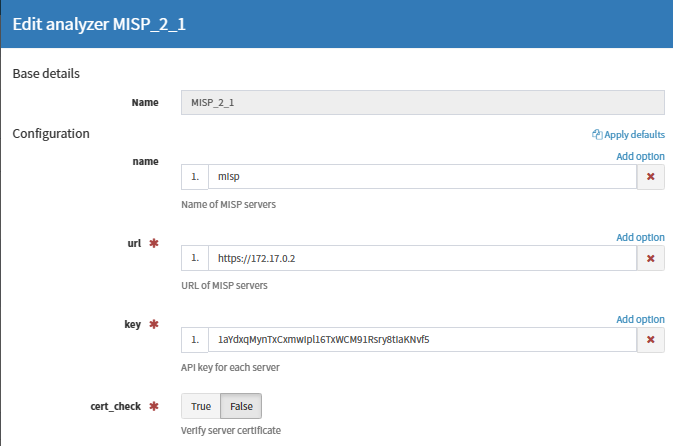
\includegraphics[width=0.9\textwidth]{images/misp_config_in_cortex.png}
    \caption{Configuration de l'integration MISP dans Cortex pour l'analyse automatisee}
    \label{fig:misp_cortex_config}
\end{figure}

Cette configuration permet l'analyse automatique des indicateurs de compromission (IOCs) extraits des alertes, enrichissant ainsi le contexte des incidents de securite avec des donnees de threat intelligence actualisees.

